\documentclass[xcolor=table]{beamer}

\usepackage{booktabs}
\usepackage{hyperref}
\usepackage[table]{xcolor}
\usepackage{tikz}
\usepackage{graphics}
\usetikzlibrary{calc, shapes}

\setbeamertemplate{navigation symbols}{}%remove navigation symbols

\title{Stochastic Games}
\subtitle{Game Theory}
\author{Vincent Knight}
\date{}

\begin{document}

\frame{\titlepage}

\frame{
\begin{itemize}
\item X a set of states with a stage game defined for each state;
\item A set of strategies $S_i(x)$ for each player for each state $x\in X$;
\item A set of rewards dependant on the state and the actions of the other players: $u_i(x,s_1,s_2)$;
\item A set of probabilities of transitioning to a future state: $\pi(x'|x,s_1,s_2)$;
\item Each stage game is played at a set of discrete times $t$.
\end{itemize}
}

\frame{
\begin{center}
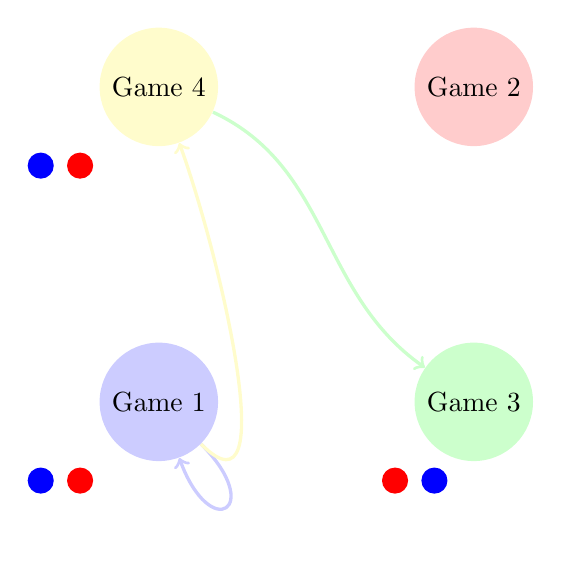
\begin{tikzpicture}
    \node (game1) at (0,0) [fill=blue!20, circle] {Game 1};
    \node (game2) at (4,4) [fill=red!20, circle] {Game 2};
    \node (game3) at (4,0) [fill=green!20, circle] {Game 3};
    \node (game4) at (0,4) [fill=yellow!20, circle] {Game 4};

    \onslide<2-5>{
    \node at (-1,-1) [fill=red, circle] {};
    \node at (-1.5,-1) [fill=blue, circle] {};
    }

    \onslide<3>{
    \draw (game1) edge[out=-45,in=-70,->,color=blue!20, very thick, looseness=9] (game1);
    }

    \onslide<5-6>{
    \draw (game1) edge[out=-45,in=-70,->,color=yellow!20, very thick] (game4);
    }

    \onslide<6-7>{
    \node at (-1,3) [fill=red, circle] {};
    \node at (-1.5,3) [fill=blue, circle] {};
    }

    \onslide<7-8>{
    \draw (game4) edge[out=-25,in=145,->,color=green!20, very thick] (game3);
    }

    \onslide<8>{
    \node at (3,-1) [fill=red, circle] {};
    \node at (3.5,-1) [fill=blue, circle] {};
    }
\end{tikzpicture}
\end{center}
}

\frame{
\tikzstyle{level 1}=[level distance=3.5cm, sibling distance=3.5cm]
\tikzstyle{level 2}=[level distance=3.5cm, sibling distance=2cm]
\tikzstyle{level 3}=[level distance=3.5cm, sibling distance=1cm]
\tikzstyle{player} = [text width=5em, draw, text centered, rectangle, fill=blue!20, inner sep=1pt]
\tikzstyle{nature} = [minimum width=3pt,circle,  draw, fill=red!20, inner sep=1pt]
\tikzstyle{end} = [circle, minimum width=3pt, fill, inner sep=0pt, right]
\begin{center}
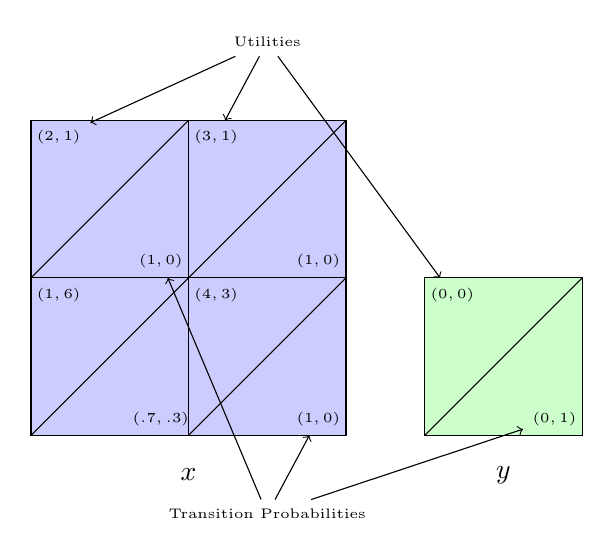
\begin{tikzpicture}
    \draw [rectangle, fill=blue!20] (0,0) -- (4,0) -- (4,4) -- (0,4) -- cycle;
    \draw (0,2) -- (4,2);
    \draw (2,0) -- (2,4);
    \draw (0,0) -- (4,4);
    \draw (0,2) -- (2,4);
    \draw (2,0) -- (4,2);
    \node (A) [right=10pt,below] at (0,4) {\tiny $(2,1)$};
    \node (B) [right=10pt,below] at (2,4) {\tiny $(3,1)$};
    \node [right=10pt,below] at (2,2) {\tiny $(4,3)$};
    \node [right=10pt,below] at (0,2) {\tiny $(1,6)$};
    \node [left=10pt,above] at (2,0) {\tiny $(.7,.3)$};
    \node [left=10pt,above] at (4,2) {\tiny $(1,0)$};
    \node (X) [left=10pt,above] at (2,2) {\tiny $(1,0)$};
    \node (Y) [left=10pt,above] at (4,0) {\tiny $(1,0)$};

    \draw [rectangle, fill=green!20] (5,0) -- (7,0) -- (7,2) -- (5,2) -- cycle;
    \draw (5,0) -- (7,2);
    \node (C) [right=10pt,below] at (5,2) {\tiny $(0,0)$};
    \node (Z) [left=10pt,above] at (7,0) {\tiny $(0,1)$};

    \node (a) at (3,5) {\tiny{Utilities}};

    \draw [->] (a) -- (A);
    \draw [->] (a) -- (B);
    \draw [->] (a) -- (C);

    \node (b) at (3,-1) {\tiny{Transition Probabilities}};

    \draw [->] (b) -- (X);
    \draw [->] (b) -- (Y);
    \draw [->] (b) -- (Z);

    \node at (2,-.5) {$x$};
    \node at (6,-.5) {$y$};
\end{tikzpicture}
\end{center}
}

\frame{

$$U_i(r,s)=\left(u_i(x,r,s)+\delta\sum_{x'\in X}\pi(x'|x,r,s)U_i^*(x')\right)$$

\pause

Thus a Nash equilibrium satisfies:

$$U_1^*(x)=\max_{r\in S_1(x)}(u_i(x,r,s^*)+\delta\sum_{x'\in X}\pi(x'|x,r,s^*)U_1^*(x')$$
$$U_2^*(x)=\max_{s\in S_2(x)}(u_i(x,r^*,s)+\delta\sum_{x'\in X}\pi(x'|x,r^*,s)U_2^*(x')$$
}


\end{document}
